% Niveau :      PCSI *
% Discipline :  Chimie Orga I
% Mots clés :   Spectrométrie UV-visible, Réactions acidobasiques

\begin{exercise}{Les hydrures du bloc $p$}{2}{Sup}
{Liaisons chimiques}{bermu}

\begin{questions}
    \questioncours Liaisons covalentes, liaisons hydrogène, liaisons Van der Waals. Analogies et différences. Comparaison des énergies associées.
    
    \question En introduisant dans le détail les concepts utilisés, commenter l'évolution des caractéristiques physiques des hydrures des éléments du bloc $p$ présentés dans la figure et la table ci-dessous.

\begin{EnvUplevel}
    \begin{figure}[H]
        \centering
        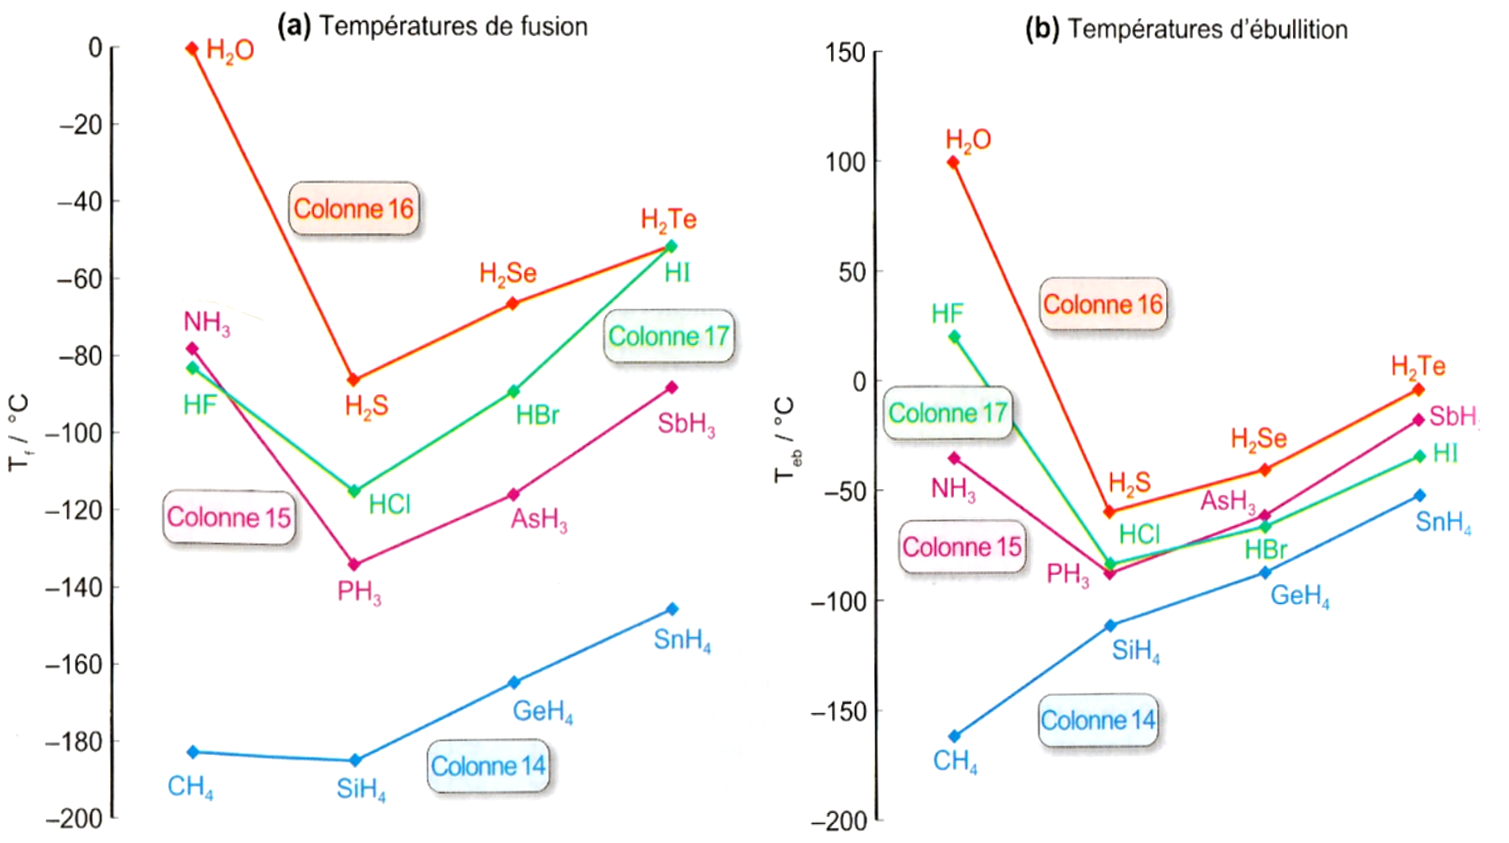
\includegraphics[width=.9\linewidth]{chimie/solvants/hydrures.png}
        \caption{Températures de fusion (a) et d'ébullition (b) des hydrures des éléments du bloc $p$ à pression atmosphérique.}
        \label{fig:hydrures}
    \end{figure}
\end{EnvUplevel}

\begin{table}[H]
    \centering
    \begin{tabularx}{.7\linewidth}{r|CCCC}
         & NH$_3$ & PH$_3$ & AsH$_3$ & SbH$_3$ \\ \hline\hline
        Solubilité vs H$_2$O (vol. / vol.) & 826 & 0,26 & 0,20 & 0,19 \\ \hline
    \end{tabularx}

    \caption{Comparaisons de propriétés chimiques des hydrures de pnictogènes (CTNP).}
    
    
\end{table}

\end{questions}

\end{exercise}

\begin{exercise}{Liasons moléculaires des nitrophénols}{2}{Sup}
{Liaisons chimiques}{bermu}

\begin{questions}

\questioncours Liaisons covalentes, liaisons hydrogène, liaisons Van der Waals. Analogies et différences. Comparaison des énergies associées.

\question En introduisant dans le détail les concepts utilisés, commenter l'évolution des caractéristiques physiques des différents nitrophénols : ortho, méta et para.
 
\begin{table}[H]  
	\setchemfig{chemfig style={scale=0.75}, atom style={scale=0.75}}
    \centering
    \begin{tabularx}{.8\linewidth}{r|CCC}
        & \chemfig{**6(---(-OH)-(-NO_3)---)}
        & \chemfig{**6(--(-OH)--(-NO_3)---)}
        & \chemfig{**6(-(-OH)---(-NO_3)---)}\\
%		& \chemfig[scale=0.75][scale=0.75]{**6(---(-OH)-(-NO_3)---)}
%       & \chemfig[scale=0.75][scale=0.75]{**6(--(-OH)--(-NO_3)---)}
%       & \chemfig[scale=0.75][scale=0.75]{**6(-(-OH)---(-NO_3)---)}\\
         & ortho & méta & para \\ \hline\hline
        Apparence & cristaux jaunes & cristaux incolores & aiguilles incolores \\
Point de fusion ($^\circ$C) & 44 & 97 & 114 \\
Point d'ébullition ($^\circ$C) & 214 & 194 & > 260 \\
pK$_a$ & 7,21 & 8,38 & 7,16 \\
Solubilité dans l'eau (g$\cdot$L$^{-1}$) & 2,1 & 13,5 & 14,8 \\ \hline
    \end{tabularx}

    \caption{Comparaisons de propriétés physiques des différents nitrophénols. (CTNP).}
\end{table}

\end{questions}

\end{exercise}